\newpage{\pagestyle{empty}\cleardoublepage}
\newpage
\vspace*{\fill}
    \begin{center}
      \thispagestyle{empty} \vspace*{0cm} \textbf{\huge
Dise\~{n}o}
    \end{center}
    \vspace*{\fill}
\newpage{\pagestyle{empty}\cleardoublepage}
\chapter{Tabla Crud}


\begin{figure}[h]
\centering
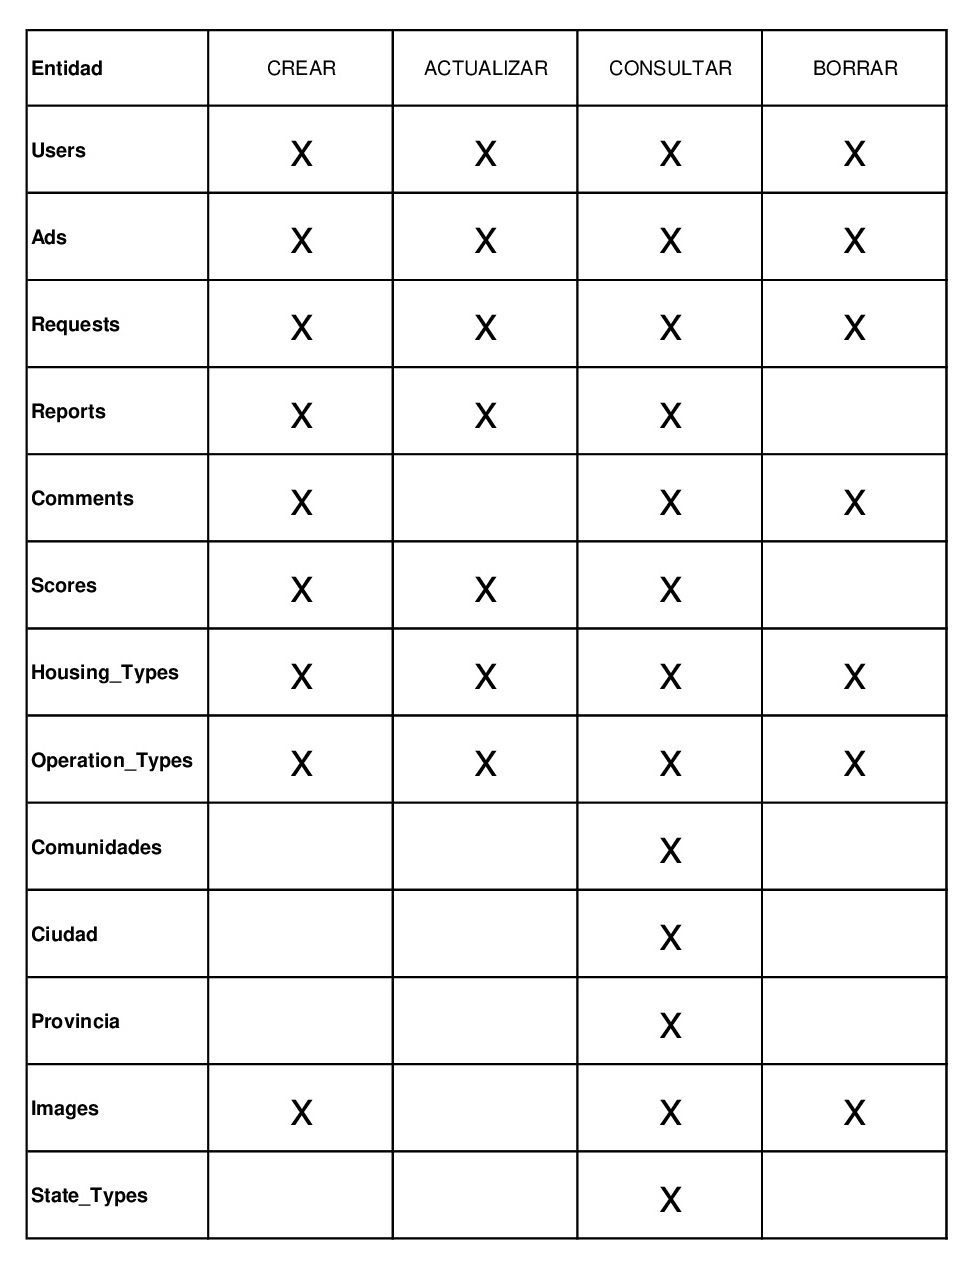
\includegraphics[width=.7\textwidth]{Img/Disenyo/TABLA_CRUD.jpg}
\caption{Tabla CRUD con las entidades y sus operaciones cubiertas.}
\label{fig:dcu}
\end{figure}

\chapter{Puntos donde se manipulan las entidades}

\section{Usuario}
\subsection{Crear}

\begin{itemize}
\item Caso 1: Registro
\begin{itemize}
\item Localizaci\'{o}n
\begin{itemize}
\item Vista: view/loginView.php
\item Controlador: controller/UserController.php
\item Modelo: model/UserModel.php
\item Dao: model/dao/UserDao.php
\item Entidad: model/dao/dto/User.php
\end{itemize}
\item Acceso: Desde la pantalla principal hacer clic en iniciar sesi\'{o}n. En la siguiente pantalla hacer clic en ''Registro''. Una vez en el formulario de alta de usuario rellenar los campos y hacer clic en el bot\'{o}n registro.
\end{itemize}

\item Caso 2: Creaci\'{o}n desde dashboard
\begin{itemize}
\item Localizaci\'{o}n
\begin{itemize}
\item Vista: view/users.php
\item Controlador: controller/AdminController.php
\item Modelo: model/UserModel.php
\item Dao: model/dao/UserDao.php
\item Entidad: model/dao/dto/User.php
\end{itemize}
\item Acceso: Desde la vista de administrador, hacer clic en la llave inglesa que nos llevar\'{a} al dashboard del sistema en la opci\'{o}n Usuarios. Hacer clic en el ''+''. Una vez se despliegue el modal , rellenar los campos y hacer clic en el bot\'{o}n enviar.
\end{itemize}
\end{itemize}

\subsection{Modificar}
\begin{itemize}
\item Caso 1: Bloqueo desde dashboard Usuarios
\begin{itemize}
\item Localizaci\'{o}n
\begin{itemize}
\item Vista: view/users.php
\item Controlador: controller/AdminController.php
\item Modelo: model/UserModel.php
\item Dao: model/dao/UserDao.php
\item Entidad: model/dao/dto/User.php
\end{itemize}
\item Acceso: Desde la vista de administrador, hacer clic en la llave inglesa que nos llevar\'{a} al dashboard del sistema en la opci\'{o}n Usuarios. Hacer clic al bot\'{o}n de la columna Ver del registro que queramos modificar para consultarlo previamente, hacemos clic en el bot\'{o}n bloquear y confirmamos en el modal haciendo clic en bloquear.
\end{itemize}
\item Caso 2: Modificaci\'{o}n desde dashboard
\begin{itemize}
\item Localizaci\'{o}n
\begin{itemize}
\item Vista: view/users.php
\item Controlador: controller/AdminController.php
\item Modelo: model/UserModel.php
\item Dao: model/dao/UserDao.php
\item Entidad: model/dao/dto/User.php
\end{itemize}
\item Acceso: Desde la vista de administrador, hacer clic en la llave inglesa que nos llevar\'{a} al dashboard del sistema en la opci\'{o}n Usuarios. Hacer clic al bot\'{o}n de la columna Ver del registro que queramos modificar para consultarlo previamente, hacemos clic en el bot\'{o}n editar y modificamos los campos del formulario. Posteriormente haremos clic en el bot\'{o}n enviar.
\end{itemize}
\item Caso 3: Aceptar denuncia sobre usuario
\begin{itemize}
\item Localizaci\'{o}n
\begin{itemize}
\item Vista: view/denuncias.php
\item Controlador: controller/AdminController.php
\item Modelo: model/UserModel.php
\item Dao: model/dao/UserDao.php
\item Entidad: model/dao/dto/User.php
\end{itemize}
\item Acceso: Desde la vista de administrador, hacer clic en la llave inglesa que nos llevar\'{a} al dashboard del sistema en la opci\'{o}n Denuncias. Hacer clic al bot\'{o}n de la columna Ver del registro para consultar la denuncia, hacemos clic en el bot\'{o}n aceptar para modificar el estado del usuario a bloqueado.
\end{itemize}
\item Caso 4: Desbloqueo desde dashboard Usuarios
\begin{itemize}
\item Localizaci\'{o}n
\begin{itemize}
\item Vista: view/users.php
\item Controlador: controller/AdminController.php
\item Modelo: model/UserModel.php
\item Dao: model/dao/UserDao.php
\item Entidad: model/dao/dto/User.php
\end{itemize}
\item Acceso: Desde la vista de administrador, hacer clic en la llave inglesa que nos llevar\'{a} al dashboard del sistema en la opci\'{o}n Usuarios. Hacer clic al bot\'{o}n de la columna Ver del registro que queramos modificar para consultarlo previamente, hacemos clic en el bot\'{o}n desbloquear y confirmamos en el modal haciendo clic en desbloquear.
\end{itemize}
\end{itemize}

\subsection{Eliminar} 
\begin{itemize}
\item Localizaci\'{o}n
\begin{itemize}
\item Vista: view/users.php
\item Controlador: controller/AdminController.php
\item Modelo: model/UserModel.php
\item Dao: model/dao/UserDao.php
\item Entidad: model/dao/dto/User.php
\end{itemize}
\item Acceso: Desde la vista de administrador, hacer clic en la llave inglesa que nos llevar\'{a} al dashboard del sistema en la opci\'{o}n Usuarios. Hacer clic al bot\'{o}n de la columna Ver del registro que queramos eliminar para consultarlo previamente, hacemos clic en el bot\'{o}n eliminar y confirmamos en el modal haciendo clic en eliminar.
\end{itemize}

\subsection{Consultar}
\begin{itemize}
\item Caso 1: Consultar desde dashboard Usuarios
\begin{itemize}
\item Localizaci\'{o}n
\begin{itemize}
\item Vista: view/users.php
\item Controlador: controller/AdminController.php - controller/WSController.php
\item Modelo: model/UserModel.php
\item Dao: model/dao/UserDao.php
\item Entidad: model/dao/dto/User.php
\end{itemize}
\item Acceso: Desde la vista de administrador, hacer clic en la llave inglesa que nos llevar\'{a} al dashboard del sistema en la opci\'{o}n Usuarios. Hacer clic al bot\'{o}n de la columna Ver del registro que queramos consultar.
\end{itemize}
\item Caso 2: Consultar desde link de usuario
\begin{itemize}
\item Localizaci\'{o}n
\begin{itemize}
\item Url: index/user/readUser\&uuid=XXXXXXXXXXX
\item Vista: view/profileView.php
\item Controlador: controller/UserController.php
\item Modelo: model/UserModel.php
\item Dao: model/dao/UserDao.php
\item Entidad: model/dao/dto/User.php
\end{itemize}
\item Acceso: Desde cualquier parte de la web desde donde se haga referencia a un usuario, se har\'{a} click en \'{e}l y este consultar\'{a} el mismo.
\end{itemize}
\end{itemize}

\section{Anuncio}
\subsection{Crear}
\begin{itemize}
\item Localizaci\'{o}n
\begin{itemize}
\item Vista: view/listAdsView.php
\item Controlador: controller/AdController.php
\item Modelo: model/AdModel.php
\item Dao: model/dao/AdDao.php
\item Entidad: model/dao/dto/Ad.php
\end{itemize}
\item Acceso: Desde cualquier p\'{a}gina hacemos click al apartado de anuncios de la cabecera del sistemas, hacemos click en el ''+'' y rellenamos los datos del formulario. Posteriormente haremos click en enviar.
\end{itemize}
\subsection{Modificar}
\begin{itemize}
\item Caso 1: Modificar desde consulta de anuncio
\begin{itemize}
\item Localizaci\'{o}n
\begin{itemize}
\item Vista: view/modifyAd.php
\item Controlador: controller/AdController.php
\item Modelo: model/AdModel.php
\item Dao: model/dao/AdDao.php
\item Entidad: model/dao/dto/Ad.php
\end{itemize}
\item Acceso: Desde el dashboard o desde la b\'{u}squeda de anuncios hacemos clic en el bot\'{o}n modificar, rellenamos los campos del formulario y hacemos click en enviar.
\end{itemize}
\item Caso 2: Bloquear anuncio
\begin{itemize}
\item Localizaci\'{o}n
\begin{itemize}
\item Vista: view/readAd.php
\item Controlador: controller/AdController.php
\item Modelo: model/AdModel.php
\item Dao: model/dao/AdDao.php
\item Entidad: model/dao/dto/Ad.php
\end{itemize}
\item Acceso: Desde el dashboard o desde la b\'{u}squeda de anuncios consultamos el anuncio deseado, hacemos clic en el bot\'{o}n bloquear y aceptamos en el modal para confirmar el bloqueo.
\end{itemize}
\item Caso 3: Desbloquear anuncio
\begin{itemize}
\item Localizaci\'{o}n
\begin{itemize}
\item Url: index/Ad/read\&uuid=XXXXXXXX
\item Vista: view/readAd.php
\item Controlador: controller/AdController.php
\item Modelo: model/AdModel.php
\item Dao: model/dao/AdDao.php
\item Entidad: model/dao/dto/Ad.php
\end{itemize}
\item Acceso: Desde el dashboard consultamos el anuncio, hacemos clic en el bot\'{o}n desbloquear.
\end{itemize}
\item Caso 4: Aceptar denuncia anuncio
\begin{itemize}
\item Localizaci\'{o}n
\begin{itemize}
\item Vista: view/denuncias.php
\item Controlador: controller/AdminController.php
\item Modelo: model/AdModel.php
\item Dao: model/dao/AdDao.php
\item Entidad: model/dao/dto/Ad.php
\end{itemize}
\item Acceso: Desde la vista de administrador, hacer clic en la llave inglesa que nos llevar\'{a} al dashboard del sistema en la opci\'{o}n Denuncias. Hacer clic al bot\'{o}n de la columna Ver del registro para consultar la denuncia, hacemos clic en el bot\'{o}n aceptar para modificar el estado del anuncio a bloqueado.
\end{itemize}
\end{itemize}

\subsection{Eliminar}
\begin{itemize}
\item Localizaci\'{o}n
\begin{itemize}
\item Url: index/Ad/read\&uuid=XXXXXXXX
\item Vista: view/readAd.php
\item Controlador: controller/AdController.php
\item Modelo: model/AdModel.php
\item Dao: model/dao/AdDao.php
\item Entidad: model/dao/dto/Ad.php
\end{itemize}
\item Acceso: Desde la vista de administrador de siendo propietario del anuncio lo consultaremos previamente, haremos click en el bot\'{o}n eliminar y confirmaremos la eliminaci\'{o}n.
\end{itemize}
\subsection{Consultar}
\begin{itemize}
\item Localizaci\'{o}n
\begin{itemize}
\item Url: index/Ad/read\&uuid=XXXXXXXX
\item Vista: view/readAd.php
\item Controlador: controller/AdController.php - controller/WSController.php 
\item Modelo: model/AdModel.php
\item Dao: model/dao/AdDao.php
\item Entidad: model/dao/dto/Ad.php
\end{itemize}
\item Acceso: Desde la vista de administrador o b\'{u}squeda de anuncios haremos click en el anuncio que queramos consultar.
\end{itemize}

\section{Peticiones}
\subsection{Crear}
\begin{itemize}
\item Localizaci\'{o}n
\begin{itemize}
\item Vista: view/readAd.php
\item Controlador: controller/RequestController.php
\item Modelo: model/RequestModel.php
\item Dao: model/dao/RequestDao.php
\item Entidad: model/dao/dto/Request.php
\end{itemize}
\item Acceso: Desde la lista de anuncios o desde el dashboard de Anuncios haremos click en consultar sobre el anuncio sobre el que queremos realizar la petici\'{o}n, posteriormente se clicar\'{a} en la opci\'{o}n estoy interesado, donde rellenaremos el formulario de la petici\'{o}n y pulsaremos en enviar.
\end{itemize}
\subsection{Modificar}
\begin{itemize}
\item Caso 1: Aceptar petici\'{o}n
\begin{itemize}
\item Localizaci\'{o}n
\begin{itemize}
\item Vista: view/profileView.php
\item Controlador: controller/RequestController.php
\item Modelo: model/RequestModel.php
\item Dao: model/dao/RequestDao.php
\item Entidad: model/dao/dto/Request.php
\end{itemize}
\item Acceso: Desde el perfil de usuario, se pulsar\'{a} en el apartado solicitudes y se consultar\'{a} la petici\'{o}n que se desea aceptar, haremos click en el bot\'{o}n del check para aceptarla.
\end{itemize}
\item Caso 2: Denegar petici\'{o}n
\begin{itemize}
\item Localizaci\'{o}n
\begin{itemize}
\item Vista: view/profileView.php
\item Controlador: controller/RequestController.php
\item Modelo: model/RequestModel.php
\item Dao: model/dao/RequestDao.php
\item Entidad: model/dao/dto/Request.php
\end{itemize}
\item Acceso: Desde el perfil de usuario, se pulsar\'{a} en el apartado solicitudes y se consultar\'{a} la petici\'{o}n que se desea denegar, haremos click en ''X''.
\end{itemize}
\end{itemize}
\subsection{Eliminar}
\begin{itemize}
\item Localizaci\'{o}n
\begin{itemize}
\item Vista: view/denuncias.php
\item Controlador: controller/AdminController.php
\item Modelo: model/RequestModel.php
\item Dao: model/dao/RequestDao.php
\item Entidad: model/dao/dto/Request.php
\end{itemize}
\item Acceso: Desde la vista de administrador, hacer clic en la llave inglesa que nos llevar\'{a} al dashboard del sistema en la opci\'{o}n Denuncias. Hacer clic al bot\'{o}n de la columna Ver del registro para consultar la denuncia, hacemos clic en el bot\'{o}n aceptar para modificar el estado de la petici\'{o}n a eliminado.
\end{itemize}
\subsection{Consultar}
\begin{itemize}
\item Localizaci\'{o}n
\begin{itemize}
\item Vista: view/profileView.php
\item Controlador: controller/RequestController.php - controller/WSController.php
\item Modelo: model/RequestModel.php
\item Dao: model/dao/RequestDao.php
\item Entidad: model/dao/dto/Request.php
\end{itemize}
\item Acceso: Desde el perfil de usuario, se pulsar\'{a} en el apartado solicitudes y se consultar\'{a} la petici\'{o}n deseada.
\end{itemize}

\section{Denuncias}
\subsection{Crear}
\begin{itemize}
\item Caso 1: Denuncia usuarios
\begin{itemize}
\item Localizaci\'{o}n
\begin{itemize}
\item Vista: view/profileView.php
\item Controlador: controller/ReportController.php
\item Modelo: model/ReportModel.php
\item Dao: model/dao/ReportDao.php
\item Entidad: model/dao/dto/Report.php
\end{itemize}
\item Acceso: Desde la consulta del usuario al c\'{u}al se quiere denunciar haremos click en denunciar. Esto nos llevar\'{a} al formulario de la denuncia que debemos rellenar y pulsar sobre el boto\'{o}n denunciar.
\end{itemize}
\item Caso 2: Denuncia anuncios
\begin{itemize}
\item Localizaci\'{o}n
\begin{itemize}
\item Url: index/Ad/read\&uuid=XXXXXXXX
\item Vista: view/readAd.php
\item Controlador: controller/ReportController.php
\item Modelo: model/ReportModel.php
\item Dao: model/dao/ReportDao.php
\item Entidad: model/dao/dto/Report.php
\end{itemize}
\item Acceso: Accedemos a la consulta del anuncio que queremos denunciar, haremos click en denunciar. Esto nos llevar\'{a} al formulario de la denuncia que debemos rellenar y pulsar sobre el boto\'{o}n denunciar. 
\end{itemize}
\item Caso 3: Denuncia comentarios
\begin{itemize}
\item Localizaci\'{o}n
\begin{itemize}
\item Url: index/Ad/read\&uuid=XXXXXXXX
\item Vista: view/readAd.php
\item Controlador: controller/ReportController.php
\item Modelo: model/ReportModel.php
\item Dao: model/dao/ReportDao.php
\item Entidad: model/dao/dto/Report.php
\end{itemize}
\item Acceso: Accedemos a la consulta de un anuncio y en la zona de comentarios haremos click en denunciar sobre el comentario que queremos denunciar, haremos click en denunciar. Esto nos llevar\'{a} al formulario de la denuncia que debemos rellenar y pulsar sobre el boto\'{o}n denunciar. 
\end{itemize}
\item Caso 4: Denuncia peticiones
\begin{itemize}
\item Localizaci\'{o}n
\begin{itemize}
\item Vista: view/profileView.php
\item Controlador: controller/ReportController.php
\item Modelo: model/ReportModel.php
\item Dao: model/dao/ReportDao.php
\item Entidad: model/dao/dto/Report.php
\end{itemize}
\item Acceso: Desde mi perfil de usuario haremos click en peticiones y en consultar la que petici\'{o}n que queramos denunciar, haremos click en denunciar. Esto nos llevar\'{a} al formulario de la denuncia que debemos rellenar y pulsar sobre el boto\'{o}n denunciar.
\end{itemize}
\end{itemize}
\subsection{Modificar}
\begin{itemize}
\item Caso 1: Aceptar denuncia
\begin{itemize}
\item Localizaci\'{o}n
\begin{itemize}
\item Vista: view/denuncias.php
\item Controller: controller/AdminController.php
\item Modelo: model/ReportModel.php
\item Dao: model/dao/ReportDao.php
\item Entidad: model/dao/dto/Report.php
\end{itemize}
\item Acceso: Desde el dashboard de denuncias, consultamos la denuncia que queramos aceptar, posteriormente haremos click en el ''check'' para aceptar la denuncia.
\end{itemize}
\item Caso 2: Denegar denuncia
\begin{itemize}
\item Localizaci\'{o}n
\begin{itemize}
\item Vista: view/denuncias.php
\item Controller: controller/AdminController.php
\item Modelo: model/ReportModel.php
\item Dao: model/dao/ReportDao.php
\item Entidad: model/dao/dto/Report.php
\end{itemize}
\item Acceso: Desde el dashboard de denuncias, consultamos la denuncia que queramos denegar, posteriormente haremos click en el ''X'' para rechazar la denuncia.
\end{itemize}
\end{itemize}
\subsection{Consultar}
\begin{itemize}
\item Localizaci\'{o}n
\begin{itemize}
\item Vista: view/denuncias.php
\item Controller: controller/AdminController.php - controller/WSController.php
\item Modelo: model/ReportModel.php
\item Dao: model/dao/ReportDao.php
\item Entidad: model/dao/dto/Report.php
\end{itemize}
\item Acceso: Desde el dashboard de denuncias se listar\'{a}n todas las denuncias sin ser atendidas, adem\'{a}s se podr\'{a}n consultar de forma m\'{a}s especifica cada denuncia haciendo click en Ver en el registro deseado.
\end{itemize}

\section{Comentarios}

\subsection{Crear}
\begin{itemize}
\item Localizaci\'{o}n
\begin{itemize}
\item Url: index/Ad/read\&uuid=XXXXXXXX
\item Vista: view/readAd.php
\item Controlador: controller/CommentController.php
\item Modelo: model/CommentModel.php
\item Dao: model/dao/CommentDao.php
\item Entidad: model/dao/dto/Comment.php
\end{itemize}
\item Acceso: Accedemos a la consulta de un anuncio y en la zona de comentarios rellenamos el campo de texto con nuestro comentario y pulsamos sobre el boto\'{o}n enviar. 
\end{itemize}
\subsection{Eliminar}
\begin{itemize}
\item Caso 1: Eliminar desde el dashboard
\begin{itemize}
\item Localizaci\'{o}n
\begin{itemize}
\item Vista: view/denuncias.php
\item Controlador: controller/AdminController.php
\item Modelo: model/CommentModel.php
\item Dao: model/dao/CommentDao.php
\item Entidad: model/dao/dto/Comment.php
\end{itemize}
\item Acceso: Desde la vista de administrador, hacer clic en la llave inglesa que nos llevar\'{a} al dashboard del sistema en la opci\'{o}n comentarios. Hacer click al bot\'{o}n de la columna Eliminar del registro para eliminarlo, haciendo click posteriormente en Eliminar del modal que nos aparecer\'{a} para confirmar.
\end{itemize}
\item Caso 2: Aceptar denuncia comentario
\begin{itemize}
\item Localizaci\'{o}n
\begin{itemize}
\item Vista: view/denuncias.php
\item Controlador: controller/AdminController.php
\item Modelo: model/CommentModel.php
\item Dao: model/dao/CommentDao.php
\item Entidad: model/dao/dto/Comment.php
\end{itemize}
\item Acceso: Desde la vista de administrador, hacer clic en la llave inglesa que nos llevar\'{a} al dashboard del sistema en la opci\'{o}n Denuncias. Hacer clic al bot\'{o}n de la columna Ver del registro para consultar la denuncia, hacemos clic en el bot\'{o}n aceptar para modificar el estado del comentario a eliminado.
\end{itemize}
\end{itemize}
\subsection{Consultar}
\begin{itemize}
\item Caso 1: Listar desde el dashboard
\begin{itemize}
\item Localizaci\'{o}n
\begin{itemize}
\item Vista: view/denuncias.php
\item Controlador: controller/AdminController.php
\item Modelo: model/CommentModel.php
\item Dao: model/dao/CommentDao.php
\item Entidad: model/dao/dto/Comment.php
\end{itemize}
\item Acceso: Desde la vista de administrador, hacer clic en la llave inglesa que nos llevar\'{a} al dashboard del sistema en la opci\'{o}n comentarios. Se nos listar\'{a}n todos los comentarios paginados.
\end{itemize}
\item Caso 2: Listar comentarios del anuncio
\begin{itemize}
\item Localizaci\'{o}n
\begin{itemize}
\item Url: index/Ad/read\&uuid=XXXXXXXX
\item Vista: view/readAd.php
\item Controlador: controller/AdController.php
\item Modelo: model/CommentModel.php
\item Dao: model/dao/CommentDao.php
\item Entidad: model/dao/dto/Comment.php
\end{itemize}
\item Acceso: Consultamos el anuncio sobre el cual queremos ver sus comentarios asociados y estos nos aparecer\'{a}n al final de la p\'{a}gina paginados.
\end{itemize}
\end{itemize}

\section{Puntuaci\'{o}n}

\subsection{Crear}
\begin{itemize}
\item Localizaci\'{o}n
\begin{itemize}
\item Url: index/Ad/read\&uuid=XXXXXXXX
\item Vista: view/readAd.php
\item Controlador: controller/ScoreController.php
\item Modelo: model/ScoreModel.php
\item Dao: model/dao/ScoreDao.php
\item Entidad: model/dao/dto/Score.php
\end{itemize}
\item Acceso: Accedemos a la consulta del anuncio que queramos puntuar, hacemos click en las manos para dar LIKE o DISLIKE.
\end{itemize}

\subsection{Modificar}
\begin{itemize}
\item Localizaci\'{o}n
\begin{itemize}
\item Url: index/Ad/read\&uuid=XXXXXXXX
\item Vista: view/readAd.php
\item Controlador: controller/ScoreController.php
\item Modelo: model/ScoreModel.php
\item Dao: model/dao/ScoreDao.php
\item Entidad: model/dao/dto/Score.php
\end{itemize}
\item Acceso: Accedemos a la consulta del anuncio que queramos modificar la puntuaci\'{o}n, hacemos click en las manos para dar LIKE o DISLIKE cambiando as\'{i} su puntuaci\'{o}n.
\end{itemize}

\subsection{Consultar}
\begin{itemize}
\item Localizaci\'{o}n
\begin{itemize}
\item Vista: view/ads.php
\item Controlador: controller/AdminController.php
\item Modelo: model/AdModel.php
\item Dao: model/dao/AdDao.php
\item Entidad: model/dao/dto/Score.php
\end{itemize}
\item Acceso: Accedemos al dashboard a las opci\'{o}n de Anuncios y se nos mostrar\'{a} el n\'{u}mero de LIKES Y DISLIKES sobre cada anuncio.
\end{itemize}